\newpage
\section{Amdahl's Law}

This section discusses Amdahl's Law, a fundamental principle in parallel computing that helps predict the theoretical speedup in latency when using multiple processors.

\subsection{Performance Metrics}
Considering $T_p$ the time to solve a problem using $p$ processors, we define:
\begin{itemize}
    \item \textbf{Speedup}: $S(p) = \frac{T_1}{T_p},\; 0 < S(p) \le p$
    \item \textbf{Efficiency}: $E(p) = \frac{S(p)}{p},\; 0 < E(p) \le 1$
\end{itemize}

\subsection{The Law}
Amdahl's Law can be expressed as a classical formula:

\[
S(p) = \frac{1}{f_s + \frac{(1-f_s)}{p}}
\]

where:
\begin{itemize}
    \item $S(p)$: is the theoretical speedup
    \item $f_s$: is the proportion of sequential code (non-parallelizable)
    \item $1-f_s$: is the proportion of parallelizable code
    \item $p$: is the number of processors
\end{itemize}

\subsubsection*{Ideal case ($f_s=0$)}
Implies that all code is parallelizable. The speedup becomes:

\[
S(p) = \frac{1}{\frac{1}{p}} = {p}
\]
\\
Maximum speedup equals the number of processors. Each processor contributes fully to the speedup.

\subsubsection*{Theoretical limit case ($p \to \infty $)}
By increasing the number of processors to infinity, the speedup reaches its theoretical limit:

\[
\lim_{p \to \infty} S(p) = \frac{1}{f_s}
\]
\\
Even tough the number of processors increases indefinitely, the speedup is limited by the sequential portion of the code, encountering a bottleneck.

\subsubsection*{Real case ($f_s=\alpha p$)}
Where $\alpha$ is a constant $\alpha <= 0.1$ representing the overhead per processor. The speedup becomes:

\[
S(p) = \frac{1}{\alpha p + \frac{1 - \alpha p}{p}} = \frac{p}{1 - \alpha p + \alpha p^2}
\]
\\
There is no free lunch: as we add more processors, the overhead increases linearly, impacting the overall speedup.

\paragraph{For $\alpha$ small:} when $\alpha$ is small we do not have a significant overhead.

\[
S(p) \approx p
\]

\paragraph{For $\alpha$ large:} when $\alpha$ is large, the overhead dominates. The more we add processors, the less benefit we get!

\[
S(p) \approx \frac{p}{\alpha p^2} \approx \frac{1}{\alpha p}
\]


\subsection{Results}
The following examples have been obtained using Matlab scripts are available in the repository (\texttt{classic\_vs\_overhead.m} and \texttt{parallel\_comparison.m}).

\subsubsection*{Classical vs Overhead}
\begin{itemize}
    \item The proportion of the parallelizable is 95\% of code.\\
    ($f_s=0.1$, $f_p = 1-f_s = 0.9$)
    \item Overhead per processor\\
    $\alpha = 0.01$
\end{itemize}

\begin{figure}[H]
    \centering
    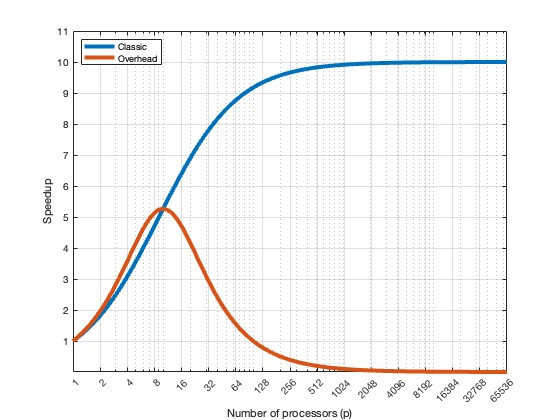
\includegraphics[width=0.7\textwidth]{assets/amdalhs_law/classic_vs_overhead.jpg}
    \label{fig:classic_vs_overhead_image}
\end{figure}

\subsubsection*{Parallel speedup comparison}
It is useful for understanding the limits of parallelization according to Amdahl's law: it highlights that simply increasing the number of processors is not enough if the sequential portion of the code is significant

\begin{figure}[H]
    \centering
    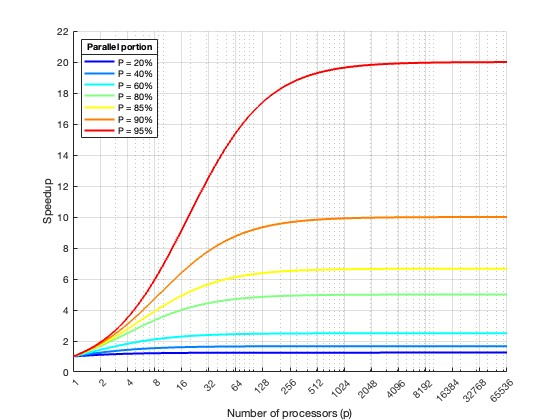
\includegraphics[width=0.8\textwidth]{assets/amdalhs_law/parallel_comparison.jpg}
    \label{fig:parallel_comparison}
\end{figure}
